%================================================================================
% PARTE 2: EJEMPLOS RESUELTOS, EJERCICIOS INVERSOS Y SOLUCIONES
%================================================================================

\section{Ejemplos Resueltos}

Ahora vamos a resolver paso a paso diferentes tipos de ecuaciones trigonométricas. Cada ejemplo te mostrará técnicas específicas que podrás aplicar en problemas similares.

\begin{ejemplo}[title=Ejemplo 1: Ecuación básica f(x) = k]
Resuelve la ecuación $\sin x = \frac{\sqrt{3}}{2}$ para $x \in [0, 2\pi]$.

\vspace{0.3cm}
\textbf{Solución:}

\textbf{Paso 1:} Identificar el ángulo de referencia.

Reconocemos que $\sin\left(\frac{\pi}{3}\right) = \frac{\sqrt{3}}{2}$, por lo tanto $\frac{\pi}{3}$ es nuestro ángulo de referencia.

\textbf{Paso 2:} Determinar en qué cuadrantes el seno es positivo.

El seno es positivo en los cuadrantes I y II (donde $y > 0$).

\textbf{Paso 3:} Encontrar las soluciones en el intervalo dado.

En el cuadrante I: $x_1 = \frac{\pi}{3}$

En el cuadrante II: $x_2 = \pi - \frac{\pi}{3} = \frac{3\pi - \pi}{3} = \frac{2\pi}{3}$

\textbf{Paso 4:} Verificación algebraica.

$\sin\left(\frac{\pi}{3}\right) = \frac{\sqrt{3}}{2}$ ✓

$\sin\left(\frac{2\pi}{3}\right) = \sin\left(\pi - \frac{\pi}{3}\right) = \sin\left(\frac{\pi}{3}\right) = \frac{\sqrt{3}}{2}$ ✓

\textbf{Paso 5:} Representación gráfica.

\begin{center}
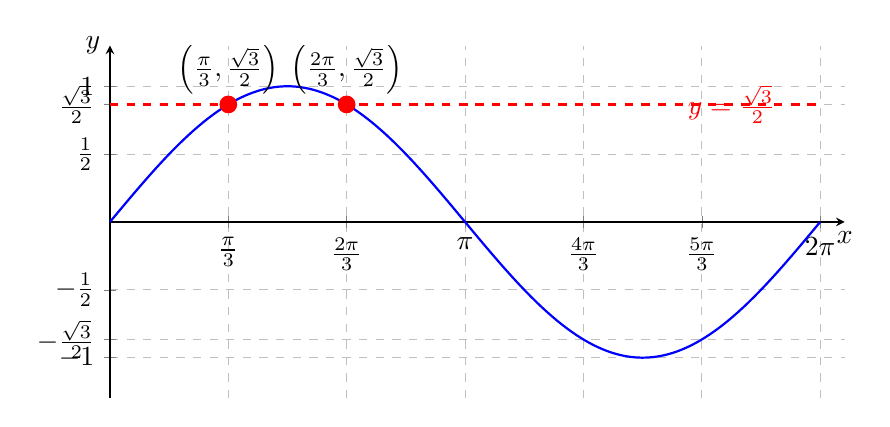
\begin{tikzpicture}
\begin{axis}[
    width=0.9\textwidth,
    height=0.5\textwidth,
    axis lines = middle,
    xlabel = {$x$},
    ylabel = {$y$},
    xlabel style={below},
    ylabel style={left},
    xmin=0, xmax=6.5,
    ymin=-1.3, ymax=1.3,
    xtick={0, 1.047, 2.094, 3.14159, 4.189, 5.236, 6.283},
    xticklabels={$0$, $\frac{\pi}{3}$, $\frac{2\pi}{3}$, $\pi$, $\frac{4\pi}{3}$, $\frac{5\pi}{3}$, $2\pi$},
    ytick={-1, -0.866, -0.5, 0, 0.5, 0.866, 1},
    yticklabels={$-1$, $-\frac{\sqrt{3}}{2}$, $-\frac{1}{2}$, $0$, $\frac{1}{2}$, $\frac{\sqrt{3}}{2}$, $1$},
    grid=major,
    grid style={dashed, gray!50},
    samples=200,
    domain=0:6.283
]
    % Función seno
    \addplot[blue, thick] {sin(deg(x))};

    % Línea horizontal y = √3/2
    \addplot[red, thick, dashed] {0.866};

    % Puntos de intersección
    \addplot[only marks, mark=*, mark size=3pt, red] coordinates {(1.047, 0.866) (2.094, 0.866)};

    % Etiquetas
    \node[above] at (axis cs:1.047, 0.866) {$\left(\frac{\pi}{3}, \frac{\sqrt{3}}{2}\right)$};
    \node[above] at (axis cs:2.094, 0.866) {$\left(\frac{2\pi}{3}, \frac{\sqrt{3}}{2}\right)$};
    \node[red] at (axis cs:5.5, 0.866) {$y = \frac{\sqrt{3}}{2}$};
\end{axis}
\end{tikzpicture}
\end{center}

\textbf{Paso 6:} Escribir el conjunto solución.

\[
\boxed{S = \left\{\frac{\pi}{3}, \frac{2\pi}{3}\right\}}
\]

\textbf{Interpretación:} La gráfica muestra que la curva del seno cruza la línea horizontal $y = \frac{\sqrt{3}}{2}$ exactamente dos veces en el intervalo $[0, 2\pi]$.
\end{ejemplo}

\begin{ejemplo}[title=Ejemplo 2: Ecuación lineal en seno]
Resuelve la ecuación $2\sin x - 1 = 0$ para $x \in [0, 360^\circ]$.

\vspace{0.3cm}
\textbf{Solución:}

\textbf{Paso 1:} Despejar la función trigonométrica.
\begin{align*}
2\sin x - 1 &= 0 \\
2\sin x &= 1 \\
\sin x &= \frac{1}{2}
\end{align*}

\textbf{Paso 2:} Identificar el ángulo de referencia.

Sabemos que $\sin(30^\circ) = \frac{1}{2}$, entonces el ángulo de referencia es $30^\circ$.

\textbf{Paso 3:} Determinar los cuadrantes donde el seno es positivo.

El seno es positivo en los cuadrantes I y II.

\textbf{Paso 4:} Encontrar todas las soluciones.

Cuadrante I: $x_1 = 30^\circ$

Cuadrante II: $x_2 = 180^\circ - 30^\circ = 150^\circ$

\textbf{Paso 5:} Verificación sustituyendo en la ecuación original.

Para $x = 30^\circ$: $2\sin(30^\circ) - 1 = 2 \cdot \frac{1}{2} - 1 = 1 - 1 = 0$ ✓

Para $x = 150^\circ$: $2\sin(150^\circ) - 1 = 2 \cdot \frac{1}{2} - 1 = 1 - 1 = 0$ ✓

\textbf{Paso 6:} Visualización en el círculo unitario.

\begin{center}
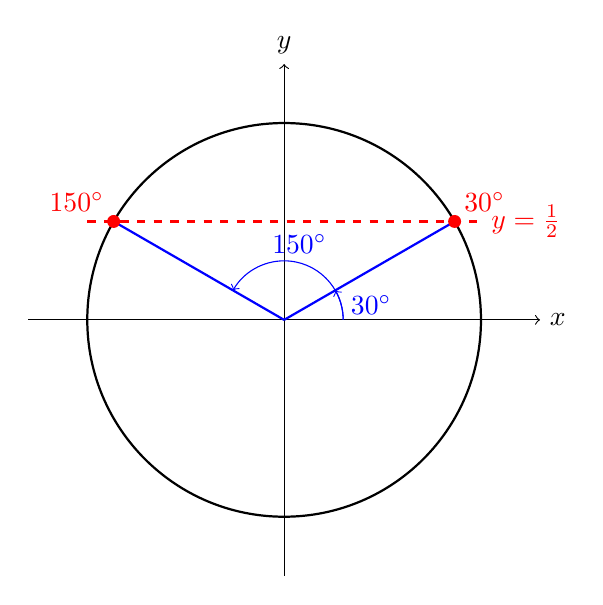
\begin{tikzpicture}[scale=2.5]
    % Círculo unitario
    \draw[thick] (0,0) circle (1);

    % Ejes
    \draw[->] (-1.3,0) -- (1.3,0) node[right] {$x$};
    \draw[->] (0,-1.3) -- (0,1.3) node[above] {$y$};

    % Línea horizontal y = 1/2
    \draw[red, thick, dashed] (-1,0.5) -- (1,0.5) node[right] {$y = \frac{1}{2}$};

    % Radios para 30° y 150°
    \draw[blue, thick] (0,0) -- (30:1);
    \draw[blue, thick] (0,0) -- (150:1);

    % Puntos de solución
    \filldraw[red] (30:1) circle (0.03) node[above right] {$30^\circ$};
    \filldraw[red] (150:1) circle (0.03) node[above left] {$150^\circ$};

    % Ángulos
    \draw[blue, ->] (0.3,0) arc (0:30:0.3) node[midway, right] {$30^\circ$};
    \draw[blue, ->] (0.3,0) arc (0:150:0.3) node[midway, above] {$150^\circ$};
\end{tikzpicture}
\end{center}

\textbf{Paso 7:} Conjunto solución.

\[
\boxed{S = \{30^\circ, 150^\circ\}}
\]
\end{ejemplo}

\begin{ejemplo}[title=Ejemplo 3: Ecuación cuadrática en coseno]
Resuelve la ecuación $2\cos^2 x - \cos x - 1 = 0$ para $x \in [0, 2\pi]$.

\vspace{0.3cm}
\textbf{Solución:}

\textbf{Paso 1:} Reconocer la forma cuadrática.

Esta es una ecuación cuadrática en $\cos x$. Hacemos la sustitución $u = \cos x$:
\[
2u^2 - u - 1 = 0
\]

\textbf{Paso 2:} Resolver la ecuación cuadrática.

Factorizando: $(2u + 1)(u - 1) = 0$

Por lo tanto: $u = -\frac{1}{2}$ o $u = 1$

\textbf{Paso 3:} Volver a la variable original.

Caso 1: $\cos x = -\frac{1}{2}$

Caso 2: $\cos x = 1$

\textbf{Paso 4:} Resolver cada caso.

\textbf{Caso 1:} $\cos x = -\frac{1}{2}$

El coseno es negativo en los cuadrantes II y III.
Ángulo de referencia: $\arccos\left(\frac{1}{2}\right) = \frac{\pi}{3}$

En el cuadrante II: $x = \pi - \frac{\pi}{3} = \frac{2\pi}{3}$

En el cuadrante III: $x = \pi + \frac{\pi}{3} = \frac{4\pi}{3}$

\textbf{Caso 2:} $\cos x = 1$

Esto ocurre cuando $x = 0$ o $x = 2\pi$

\textbf{Paso 5:} Verificación.

Para $x = 0$: $2\cos^2(0) - \cos(0) - 1 = 2(1) - 1 - 1 = 0$ ✓

Para $x = \frac{2\pi}{3}$: $2\left(-\frac{1}{2}\right)^2 - \left(-\frac{1}{2}\right) - 1 = \frac{1}{2} + \frac{1}{2} - 1 = 0$ ✓

Para $x = \frac{4\pi}{3}$: $2\left(-\frac{1}{2}\right)^2 - \left(-\frac{1}{2}\right) - 1 = \frac{1}{2} + \frac{1}{2} - 1 = 0$ ✓

Para $x = 2\pi$: $2\cos^2(2\pi) - \cos(2\pi) - 1 = 2(1) - 1 - 1 = 0$ ✓

\textbf{Paso 6:} Representación gráfica.

\begin{center}
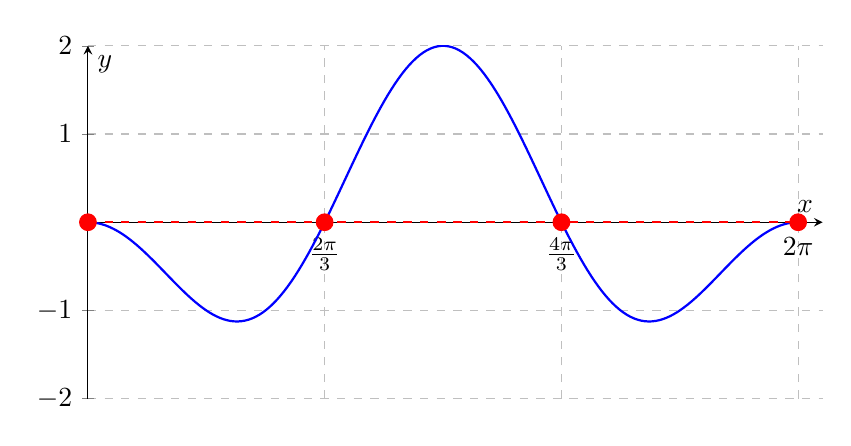
\begin{tikzpicture}
\begin{axis}[
    width=0.9\textwidth,
    height=0.5\textwidth,
    axis lines = middle,
    xlabel = {$x$},
    ylabel = {$y$},
    xmin=0, xmax=6.5,
    ymin=-2, ymax=2,
    xtick={0, 2.094, 4.189, 6.283},
    xticklabels={$0$, $\frac{2\pi}{3}$, $\frac{4\pi}{3}$, $2\pi$},
    grid=major,
    grid style={dashed, gray!50},
    samples=200,
    domain=0:6.283
]
    % Función 2cos²x - cosx - 1
    \addplot[blue, thick] {2*cos(deg(x))^2 - cos(deg(x)) - 1};

    % Línea y = 0
    \addplot[red, thick, dashed] {0};

    % Puntos de intersección
    \addplot[only marks, mark=*, mark size=3pt, red] coordinates {(0, 0) (2.094, 0) (4.189, 0) (6.283, 0)};
\end{axis}
\end{tikzpicture}
\end{center}

\textbf{Paso 7:} Conjunto solución.

\[
\boxed{S = \left\{0, \frac{2\pi}{3}, \frac{4\pi}{3}, 2\pi\right\}}
\]
\end{ejemplo}

\begin{ejemplo}[title=Ejemplo 4: Ecuación con identidad fundamental]
Resuelve la ecuación $\sin^2 x + \sin x = 2 - 2\cos^2 x$ para $x \in [0, 2\pi]$.

\vspace{0.3cm}
\textbf{Solución:}

\textbf{Paso 1:} Usar la identidad fundamental $\sin^2 x + \cos^2 x = 1$.

De esta identidad: $\cos^2 x = 1 - \sin^2 x$

\textbf{Paso 2:} Sustituir en la ecuación original.
\begin{align*}
\sin^2 x + \sin x &= 2 - 2\cos^2 x \\
\sin^2 x + \sin x &= 2 - 2(1 - \sin^2 x) \\
\sin^2 x + \sin x &= 2 - 2 + 2\sin^2 x \\
\sin^2 x + \sin x &= 2\sin^2 x
\end{align*}

\textbf{Paso 3:} Simplificar y reorganizar.
\begin{align*}
\sin^2 x + \sin x - 2\sin^2 x &= 0 \\
-\sin^2 x + \sin x &= 0 \\
\sin x(1 - \sin x) &= 0
\end{align*}

\textbf{Paso 4:} Resolver cada factor.

Factor 1: $\sin x = 0$
Soluciones: $x = 0, \pi, 2\pi$

Factor 2: $1 - \sin x = 0 \Rightarrow \sin x = 1$
Solución: $x = \frac{\pi}{2}$

\textbf{Paso 5:} Verificación con la ecuación original.

Para $x = 0$:
$\sin^2(0) + \sin(0) = 0 + 0 = 0$
$2 - 2\cos^2(0) = 2 - 2(1) = 0$ ✓

Para $x = \frac{\pi}{2}$:
$\sin^2\left(\frac{\pi}{2}\right) + \sin\left(\frac{\pi}{2}\right) = 1 + 1 = 2$
$2 - 2\cos^2\left(\frac{\pi}{2}\right) = 2 - 2(0) = 2$ ✓

Para $x = \pi$:
$\sin^2(\pi) + \sin(\pi) = 0 + 0 = 0$
$2 - 2\cos^2(\pi) = 2 - 2(1) = 0$ ✓

Para $x = 2\pi$:
$\sin^2(2\pi) + \sin(2\pi) = 0 + 0 = 0$
$2 - 2\cos^2(2\pi) = 2 - 2(1) = 0$ ✓

\textbf{Paso 6:} Representación en el círculo unitario.

\begin{center}
\begin{tikzpicture}[scale=2.5]
    % Círculo unitario
    \draw[thick] (0,0) circle (1);

    % Ejes
    \draw[->] (-1.3,0) -- (1.3,0) node[right] {$x$};
    \draw[->] (0,-1.3) -- (0,1.3) node[above] {$y$};

    % Puntos solución
    \filldraw[red] (1,0) circle (0.03) node[below right] {$0, 2\pi$};
    \filldraw[red] (0,1) circle (0.03) node[above right] {$\frac{\pi}{2}$};
    \filldraw[red] (-1,0) circle (0.03) node[below left] {$\pi$};

    % Radios
    \draw[blue, thick] (0,0) -- (1,0);
    \draw[blue, thick] (0,0) -- (0,1);
    \draw[blue, thick] (0,0) -- (-1,0);
\end{tikzpicture}
\end{center}

\textbf{Paso 7:} Conjunto solución.

\[
\boxed{S = \left\{0, \frac{\pi}{2}, \pi, 2\pi\right\}}
\]
\end{ejemplo}

\begin{ejemplo}[title=Ejemplo 5: Ecuación con ángulo doble]
Resuelve la ecuación $\sin(2x) = \cos x$ para $x \in [0, 2\pi]$.

\vspace{0.3cm}
\textbf{Solución:}

\textbf{Paso 1:} Aplicar la fórmula del ángulo doble.

Recordemos que $\sin(2x) = 2\sin x \cos x$

\textbf{Paso 2:} Sustituir en la ecuación.
\begin{align*}
2\sin x \cos x &= \cos x \\
2\sin x \cos x - \cos x &= 0 \\
\cos x(2\sin x - 1) &= 0
\end{align*}

\textbf{Paso 3:} Resolver cada factor.

\textbf{Factor 1:} $\cos x = 0$
Soluciones: $x = \frac{\pi}{2}, \frac{3\pi}{2}$

\textbf{Factor 2:} $2\sin x - 1 = 0 \Rightarrow \sin x = \frac{1}{2}$
Soluciones: $x = \frac{\pi}{6}, \frac{5\pi}{6}$

\textbf{Paso 4:} Verificación con la ecuación original.

Para $x = \frac{\pi}{6}$:
$\sin\left(2 \cdot \frac{\pi}{6}\right) = \sin\left(\frac{\pi}{3}\right) = \frac{\sqrt{3}}{2}$
$\cos\left(\frac{\pi}{6}\right) = \frac{\sqrt{3}}{2}$ ✓

Para $x = \frac{\pi}{2}$:
$\sin\left(2 \cdot \frac{\pi}{2}\right) = \sin(\pi) = 0$
$\cos\left(\frac{\pi}{2}\right) = 0$ ✓

Para $x = \frac{5\pi}{6}$:
$\sin\left(2 \cdot \frac{5\pi}{6}\right) = \sin\left(\frac{5\pi}{3}\right) = -\frac{\sqrt{3}}{2}$
$\cos\left(\frac{5\pi}{6}\right) = -\frac{\sqrt{3}}{2}$ ✓

Para $x = \frac{3\pi}{2}$:
$\sin\left(2 \cdot \frac{3\pi}{2}\right) = \sin(3\pi) = 0$
$\cos\left(\frac{3\pi}{2}\right) = 0$ ✓

\textbf{Paso 5:} Gráfica de ambas funciones.

\begin{center}
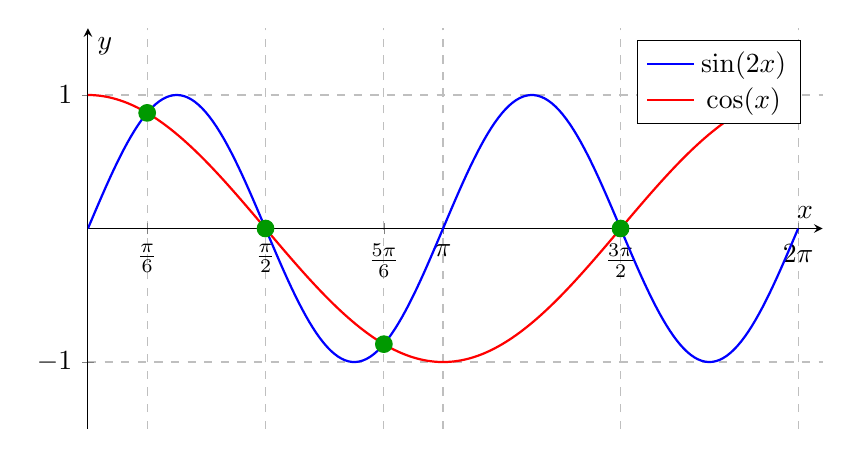
\begin{tikzpicture}
\begin{axis}[
    width=0.9\textwidth,
    height=0.55\textwidth,
    axis lines = middle,
    xlabel = {$x$},
    ylabel = {$y$},
    xmin=0, xmax=6.5,
    ymin=-1.5, ymax=1.5,
    xtick={0, 0.524, 1.571, 2.618, 3.14159, 4.712, 6.283},
    xticklabels={$0$, $\frac{\pi}{6}$, $\frac{\pi}{2}$, $\frac{5\pi}{6}$, $\pi$, $\frac{3\pi}{2}$, $2\pi$},
    grid=major,
    grid style={dashed, gray!50},
    samples=200,
    domain=0:6.283,
    legend pos=north east
]
    % sin(2x)
    \addplot[blue, thick] {sin(2*deg(x))};
    \addlegendentry{$\sin(2x)$}

    % cos(x)
    \addplot[red, thick] {cos(deg(x))};
    \addlegendentry{$\cos(x)$}

    % Puntos de intersección
    \addplot[only marks, mark=*, mark size=3pt, green!60!black]
        coordinates {(0.524, 0.866) (1.571, 0) (2.618, -0.866) (4.712, 0)};
\end{axis}
\end{tikzpicture}
\end{center}

\textbf{Paso 6:} Conjunto solución.

\[
\boxed{S = \left\{\frac{\pi}{6}, \frac{\pi}{2}, \frac{5\pi}{6}, \frac{3\pi}{2}\right\}}
\]
\end{ejemplo}

\begin{ejemplo}[title=Ejemplo 6: Ecuación con ángulo medio]
Resuelve la ecuación $\cos\left(\frac{x}{2}\right) = \sin x$ para $x \in [0, 2\pi]$.

\vspace{0.3cm}
\textbf{Solución:}

\textbf{Paso 1:} Usar la identidad del ángulo medio y doble.

Sabemos que $\sin x = 2\sin\left(\frac{x}{2}\right)\cos\left(\frac{x}{2}\right)$

\textbf{Paso 2:} Sustituir en la ecuación.
\begin{align*}
\cos\left(\frac{x}{2}\right) &= 2\sin\left(\frac{x}{2}\right)\cos\left(\frac{x}{2}\right) \\
\cos\left(\frac{x}{2}\right) - 2\sin\left(\frac{x}{2}\right)\cos\left(\frac{x}{2}\right) &= 0 \\
\cos\left(\frac{x}{2}\right)\left[1 - 2\sin\left(\frac{x}{2}\right)\right] &= 0
\end{align*}

\textbf{Paso 3:} Resolver cada factor.

\textbf{Factor 1:} $\cos\left(\frac{x}{2}\right) = 0$

Esto ocurre cuando $\frac{x}{2} = \frac{\pi}{2} + n\pi$

Para $n = 0$: $\frac{x}{2} = \frac{\pi}{2} \Rightarrow x = \pi$

\textbf{Factor 2:} $1 - 2\sin\left(\frac{x}{2}\right) = 0 \Rightarrow \sin\left(\frac{x}{2}\right) = \frac{1}{2}$

Esto ocurre cuando $\frac{x}{2} = \frac{\pi}{6}$ o $\frac{x}{2} = \frac{5\pi}{6}$

Por lo tanto: $x = \frac{\pi}{3}$ o $x = \frac{5\pi}{3}$

\textbf{Paso 4:} Verificación.

Para $x = \frac{\pi}{3}$:
$\cos\left(\frac{\pi}{6}\right) = \frac{\sqrt{3}}{2}$
$\sin\left(\frac{\pi}{3}\right) = \frac{\sqrt{3}}{2}$ ✓

Para $x = \pi$:
$\cos\left(\frac{\pi}{2}\right) = 0$
$\sin(\pi) = 0$ ✓

Para $x = \frac{5\pi}{3}$:
$\cos\left(\frac{5\pi}{6}\right) = -\frac{\sqrt{3}}{2}$
$\sin\left(\frac{5\pi}{3}\right) = -\frac{\sqrt{3}}{2}$ ✓

\textbf{Paso 5:} Visualización gráfica.

\begin{center}
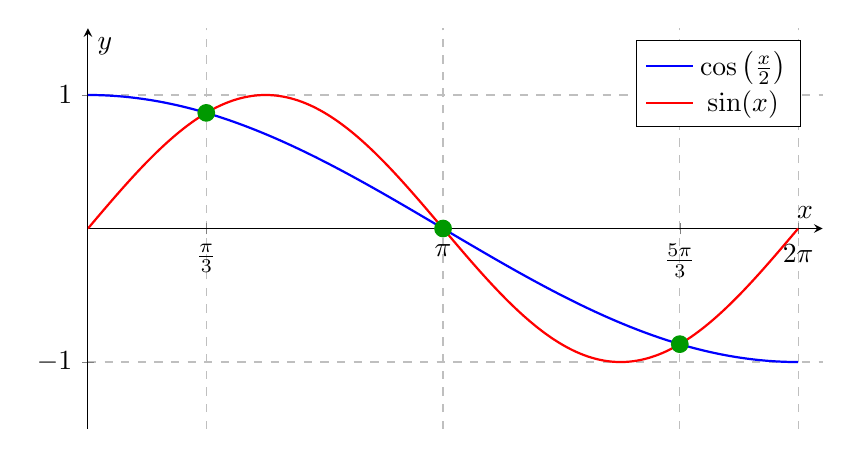
\begin{tikzpicture}
\begin{axis}[
    width=0.9\textwidth,
    height=0.55\textwidth,
    axis lines = middle,
    xlabel = {$x$},
    ylabel = {$y$},
    xmin=0, xmax=6.5,
    ymin=-1.5, ymax=1.5,
    xtick={0, 1.047, 3.14159, 5.236, 6.283},
    xticklabels={$0$, $\frac{\pi}{3}$, $\pi$, $\frac{5\pi}{3}$, $2\pi$},
    grid=major,
    grid style={dashed, gray!50},
    samples=200,
    domain=0:6.283,
    legend pos=north east
]
    % cos(x/2)
    \addplot[blue, thick] {cos(deg(x/2))};
    \addlegendentry{$\cos\left(\frac{x}{2}\right)$}

    % sin(x)
    \addplot[red, thick] {sin(deg(x))};
    \addlegendentry{$\sin(x)$}

    % Puntos de intersección
    \addplot[only marks, mark=*, mark size=3pt, green!60!black]
        coordinates {(1.047, 0.866) (3.14159, 0) (5.236, -0.866)};
\end{axis}
\end{tikzpicture}
\end{center}

\textbf{Paso 6:} Conjunto solución.

\[
\boxed{S = \left\{\frac{\pi}{3}, \pi, \frac{5\pi}{3}\right\}}
\]
\end{ejemplo}

\begin{ejemplo}[title=Ejemplo 7: Ecuación con función inversa]
Resuelve la ecuación $\arcsin(x) = \arccos(2x)$ para $x \in \mathbb{R}$.

\vspace{0.3cm}
\textbf{Solución:}

\textbf{Paso 1:} Determinar el dominio.

Para $\arcsin(x)$: $-1 \leq x \leq 1$

Para $\arccos(2x)$: $-1 \leq 2x \leq 1 \Rightarrow -\frac{1}{2} \leq x \leq \frac{1}{2}$

Dominio común: $x \in \left[-\frac{1}{2}, \frac{1}{2}\right]$

\textbf{Paso 2:} Aplicar una función trigonométrica a ambos lados.

Sea $\theta = \arcsin(x) = \arccos(2x)$

Entonces: $\sin\theta = x$ y $\cos\theta = 2x$

\textbf{Paso 3:} Usar la identidad fundamental.
\begin{align*}
\sin^2\theta + \cos^2\theta &= 1 \\
x^2 + (2x)^2 &= 1 \\
x^2 + 4x^2 &= 1 \\
5x^2 &= 1 \\
x^2 &= \frac{1}{5} \\
x &= \pm\frac{1}{\sqrt{5}} = \pm\frac{\sqrt{5}}{5}
\end{align*}

\textbf{Paso 4:} Verificar cuál solución es válida.

Para $x = \frac{\sqrt{5}}{5} \approx 0.447$:

$\arcsin\left(\frac{\sqrt{5}}{5}\right) \approx 0.464$ radianes

$\arccos\left(\frac{2\sqrt{5}}{5}\right) \approx 0.464$ radianes ✓

Para $x = -\frac{\sqrt{5}}{5}$:

$\arcsin\left(-\frac{\sqrt{5}}{5}\right) \approx -0.464$ radianes

$\arccos\left(-\frac{2\sqrt{5}}{5}\right) \approx 2.678$ radianes ✗

\textbf{Paso 5:} Verificación adicional.

Necesitamos que $\sin\theta = x$ y $\cos\theta = 2x$ con el mismo $\theta$.

Para $x = \frac{\sqrt{5}}{5}$:
- Si $\sin\theta = \frac{\sqrt{5}}{5}$, entonces $\theta \approx 26.57^\circ$
- Si $\cos\theta = \frac{2\sqrt{5}}{5}$, entonces $\theta \approx 26.57^\circ$ ✓

\textbf{Paso 6:} Representación gráfica.

\begin{center}
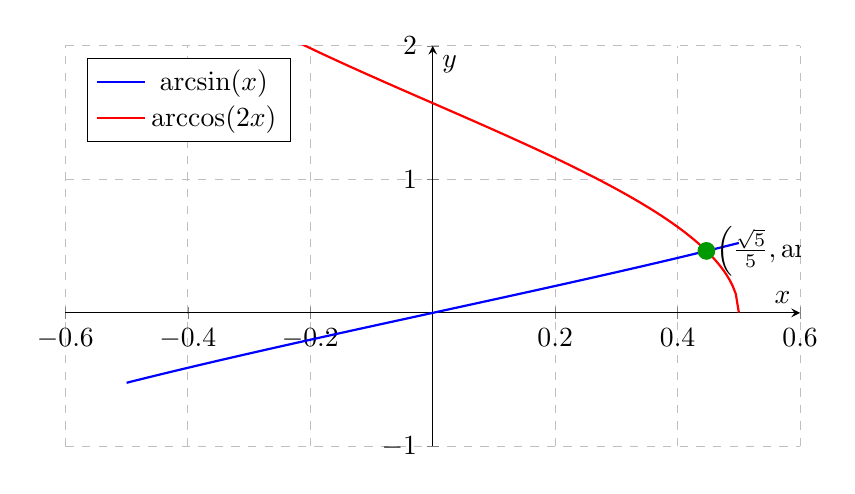
\begin{tikzpicture}
\begin{axis}[
    width=0.9\textwidth,
    height=0.55\textwidth,
    axis lines = middle,
    xlabel = {$x$},
    ylabel = {$y$},
    xmin=-0.6, xmax=0.6,
    ymin=-1, ymax=2,
    grid=major,
    grid style={dashed, gray!50},
    samples=200,
    domain=-0.5:0.5,
    legend pos=north west
]
    % arcsin(x)
    \addplot[blue, thick, domain=-0.5:0.5] {rad(asin(x))};
    \addlegendentry{$\arcsin(x)$}

    % arccos(2x)
    \addplot[red, thick, domain=-0.5:0.5] {rad(acos(2*x))};
    \addlegendentry{$\arccos(2x)$}

    % Punto de intersección
    \addplot[only marks, mark=*, mark size=3pt, green!60!black]
        coordinates {(0.447, 0.464)};

    \node[right] at (axis cs:0.447, 0.464) {$\left(\frac{\sqrt{5}}{5}, \arcsin\left(\frac{\sqrt{5}}{5}\right)\right)$};
\end{axis}
\end{tikzpicture}
\end{center}

\textbf{Paso 7:} Solución.

\[
\boxed{x = \frac{\sqrt{5}}{5}}
\]
\end{ejemplo}

\begin{ejemplo}[title=Ejemplo 8: Aplicación - Dirección de un carro en curva]
Un carro recorre una pista circular de radio 50 metros. La dirección del carro (ángulo que forma con el eje horizontal) en función del tiempo está dada por $\theta(t) = \frac{\pi t}{6}$ radianes, donde $t$ está en segundos. Si el carro debe apuntar hacia un punto fijo ubicado en $(100, 0)$ metros, ¿en qué momentos durante los primeros 12 segundos el carro apunta exactamente hacia ese punto?

\vspace{0.3cm}
\textbf{Solución:}

\textbf{Paso 1:} Establecer la posición del carro.

En el tiempo $t$, el carro está en:
\[
(x(t), y(t)) = (50\cos\theta(t), 50\sin\theta(t)) = \left(50\cos\left(\frac{\pi t}{6}\right), 50\sin\left(\frac{\pi t}{6}\right)\right)
\]

\textbf{Paso 2:} Determinar el vector de dirección hacia el punto objetivo.

Vector desde el carro hasta $(100, 0)$:
\[
\vec{v} = (100 - 50\cos\left(\frac{\pi t}{6}\right), -50\sin\left(\frac{\pi t}{6}\right))
\]

\textbf{Paso 3:} Calcular el ángulo de este vector.

El ángulo que forma este vector con el eje horizontal es:
\[
\alpha = \arctan\left(\frac{-50\sin\left(\frac{\pi t}{6}\right)}{100 - 50\cos\left(\frac{\pi t}{6}\right)}\right)
\]

\textbf{Paso 4:} Condición para que el carro apunte al objetivo.

El carro apunta en la dirección tangente al círculo, que forma un ángulo de $\theta(t) + \frac{\pi}{2}$ con el eje horizontal.

Para que apunte al objetivo: la dirección tangente debe ser paralela al vector hacia el objetivo.

Esto ocurre cuando el vector hacia el objetivo es perpendicular al radio, es decir, cuando:
\[
(100 - 50\cos\theta) \cdot 50\cos\theta + (-50\sin\theta) \cdot 50\sin\theta = 0
\]

\textbf{Paso 5:} Simplificar la ecuación.
\begin{align*}
50\cos\theta(100 - 50\cos\theta) - 2500\sin^2\theta &= 0 \\
5000\cos\theta - 2500\cos^2\theta - 2500\sin^2\theta &= 0 \\
5000\cos\theta - 2500(\cos^2\theta + \sin^2\theta) &= 0 \\
5000\cos\theta - 2500 &= 0 \\
\cos\theta &= \frac{1}{2}
\end{align*}

\textbf{Paso 6:} Resolver para $t$.

$\cos\left(\frac{\pi t}{6}\right) = \frac{1}{2}$

Esto ocurre cuando $\frac{\pi t}{6} = \frac{\pi}{3} + 2n\pi$ o $\frac{\pi t}{6} = -\frac{\pi}{3} + 2n\pi$

Primera familia: $t = 2 + 12n$

Segunda familia: $t = -2 + 12n$ (pero $t \geq 0$, así que $t = 10$ para $n = 1$)

\textbf{Paso 7:} Soluciones en $[0, 12]$ segundos.

$t = 2$ segundos y $t = 10$ segundos

\textbf{Paso 8:} Verificación y visualización.

\begin{center}
\begin{tikzpicture}[scale=0.06]
    % Pista circular
    \draw[thick] (0,0) circle (50);

    % Punto objetivo
    \filldraw[red] (100,0) circle (1.5) node[above] {Objetivo};

    % Posición en t=2 (ángulo π/3)
    \coordinate (P1) at (60:50);
    \filldraw[blue] (P1) circle (1.5);
    \draw[blue, thick, ->] (P1) -- ++(150:20) node[above] {$t=2s$};
    \draw[green, dashed] (P1) -- (100,0);

    % Posición en t=10 (ángulo 5π/3)
    \coordinate (P2) at (300:50);
    \filldraw[blue] (P2) circle (1.5);
    \draw[blue, thick, ->] (P2) -- ++(30:20) node[right] {$t=10s$};
    \draw[green, dashed] (P2) -- (100,0);

    % Centro
    \filldraw (0,0) circle (1) node[below] {Centro};

    % Ejes
    \draw[->] (-60,0) -- (110,0) node[right] {$x$};
    \draw[->] (0,-60) -- (0,60) node[above] {$y$};
\end{tikzpicture}
\end{center}

\[
\boxed{\text{El carro apunta al objetivo en } t = 2 \text{ segundos y } t = 10 \text{ segundos}}
\]
\end{ejemplo}

\newpage

\section{Ejercicios Inversos Creativos}

Los siguientes ejercicios requieren que apliques las ecuaciones trigonométricas de manera creativa para resolver problemas del mundo real. No te preocupes si parecen difíciles al principio, las soluciones detalladas están en la siguiente sección.

\begin{ejercicio}[title=Ejercicio Creativo 1: Navegación Marítima]
Un barco navega en línea recta desde el puerto A hacia el puerto B. Sin embargo, una corriente marina desvía su trayectoria según la ecuación:
\[
d(t) = 10\sin\left(\frac{\pi t}{6}\right) + 5\cos\left(\frac{\pi t}{3}\right)
\]
donde $d(t)$ es la desviación lateral en kilómetros y $t$ es el tiempo en horas.

El capitán necesita saber cuándo el barco estará exactamente en la línea recta original (sin desviación) durante las primeras 12 horas de viaje. Encuentra todos los momentos en que $d(t) = 0$.

\textit{Pista: Puedes usar la identidad $\cos(2\alpha) = 1 - 2\sin^2(\alpha)$ para simplificar.}
\end{ejercicio}

\begin{ejercicio}[title=Ejercicio Creativo 2: Interferencia de Ondas de Radio]
Dos torres de radio emiten señales que interfieren entre sí. La intensidad resultante en un punto está dada por:
\[
I(x) = 4\cos^2\left(\frac{2\pi x}{\lambda}\right) + 4\sin\left(\frac{2\pi x}{\lambda}\right)\cos\left(\frac{2\pi x}{\lambda}\right) + 1
\]
donde $x$ es la distancia desde la primera torre y $\lambda = 100$ metros es la longitud de onda.

Un ingeniero necesita ubicar los puntos de máxima intensidad (donde $I(x) = 5$) en el intervalo $[0, 200]$ metros. Encuentra todas las posiciones $x$ donde esto ocurre.

\textit{Pista: Usa la identidad del ángulo doble para el seno.}
\end{ejercicio}

\begin{ejercicio}[title=Ejercicio Creativo 3: Sistema de Poleas Sincronizadas]
En una fábrica, dos poleas están conectadas por una correa. La polea A tiene radio 30 cm y gira con velocidad angular $\omega_A = 2$ rad/s. La polea B tiene radio 20 cm. La posición angular de cada polea está dada por:
- Polea A: $\theta_A(t) = 2t + \frac{\pi}{4}$
- Polea B: $\theta_B(t) = 3t - \frac{\pi}{6}$

Para evitar que la correa se deslice, las poleas deben estar sincronizadas de modo que:
\[
\sin(\theta_A - \theta_B) = \frac{1}{2}
\]

¿En qué momentos durante el primer minuto ($t \in [0, 60]$ segundos) se cumple esta condición de sincronización?
\end{ejercicio}

\begin{ejercicio}[title=Ejercicio Creativo 4: Telescopio Espacial]
Un telescopio espacial debe mantener su orientación para observar una estrella distante. La orientación del telescopio varía debido a perturbaciones según:
\[
\alpha(t) = 0.1\sin(t) + 0.05\cos(2t)
\]
donde $\alpha(t)$ es el ángulo de desviación en radianes y $t$ es el tiempo en horas.

El telescopio puede tomar fotografías útiles solo cuando $|\alpha(t)| < 0.05$ radianes. Además, por restricciones de energía, solo puede operar cuando $\cos(t) > 0$.

Encuentra los intervalos de tiempo en $[0, 2\pi]$ horas donde el telescopio puede tomar fotografías útiles.

\textit{Pista: Esta es una desigualdad trigonométrica. Analiza los casos por separado.}
\end{ejercicio}

\begin{ejercicio}[title=Ejercicio Creativo 5: Resonancia en un Puente]
Un puente colgante oscila bajo la acción del viento. La amplitud de oscilación en función de la frecuencia del viento está dada por:
\[
A(f) = \frac{10}{|4 - \tan^2(\pi f)|}
\]
donde $f$ es la frecuencia en Hz y $A(f)$ es la amplitud en metros.

Por seguridad, la amplitud debe mantenerse menor a 2 metros. El puente entra en resonancia peligrosa cuando $A(f) = \infty$ (el denominador se hace cero).

a) Encuentra todas las frecuencias de resonancia en el intervalo $f \in (0, 1)$ Hz.

b) Determina los intervalos de frecuencia seguros donde $A(f) < 2$ metros.

\textit{Nota: Ten cuidado con las asíntotas verticales donde ocurre la resonancia.}
\end{ejercicio}

\newpage

\section{Soluciones de Ejercicios Inversos Creativos}

\begin{solucion}[title=Solución Ejercicio Creativo 1: Navegación Marítima]
\textbf{Encontrar:} Momentos donde $d(t) = 0$ en $[0, 12]$ horas.

\textbf{Ecuación:} $10\sin\left(\frac{\pi t}{6}\right) + 5\cos\left(\frac{\pi t}{3}\right) = 0$

\textbf{Paso 1:} Simplificar usando la relación entre los argumentos.

Notemos que $\frac{\pi t}{3} = 2 \cdot \frac{\pi t}{6}$

Sea $u = \frac{\pi t}{6}$, entonces la ecuación se convierte en:
\[
10\sin u + 5\cos(2u) = 0
\]

\textbf{Paso 2:} Aplicar la identidad del ángulo doble.

$\cos(2u) = 1 - 2\sin^2 u$

Sustituyendo:
\begin{align*}
10\sin u + 5(1 - 2\sin^2 u) &= 0 \\
10\sin u + 5 - 10\sin^2 u &= 0 \\
-10\sin^2 u + 10\sin u + 5 &= 0 \\
-2\sin^2 u + 2\sin u + 1 &= 0 \\
2\sin^2 u - 2\sin u - 1 &= 0
\end{align*}

\textbf{Paso 3:} Resolver la ecuación cuadrática.

Usando la fórmula cuadrática con $a = 2$, $b = -2$, $c = -1$:
\[
\sin u = \frac{2 \pm \sqrt{4 + 8}}{4} = \frac{2 \pm 2\sqrt{3}}{4} = \frac{1 \pm \sqrt{3}}{2}
\]

Como $-1 \leq \sin u \leq 1$:
- $\sin u = \frac{1 + \sqrt{3}}{2} \approx 1.366$ (imposible)
- $\sin u = \frac{1 - \sqrt{3}}{2} \approx -0.366$

\textbf{Paso 4:} Encontrar los valores de $u$.

$\sin u = \frac{1 - \sqrt{3}}{2} \approx -0.366$

$u = \arcsin(-0.366) \approx -0.375$ rad o $u = \pi - \arcsin(-0.366) \approx 3.517$ rad

Como $u = \frac{\pi t}{6}$ y necesitamos $t \in [0, 12]$:
- $u \in [0, 2\pi]$

Las soluciones en este intervalo son:
- $u_1 = \pi + \arcsin(0.366) \approx 3.517$ rad
- $u_2 = 2\pi - \arcsin(0.366) \approx 5.908$ rad

\textbf{Paso 5:} Convertir a tiempo.

$t = \frac{6u}{\pi}$

- $t_1 = \frac{6 \cdot 3.517}{\pi} \approx 6.72$ horas
- $t_2 = \frac{6 \cdot 5.908}{\pi} \approx 11.28$ horas

\textbf{Paso 6:} Verificación gráfica.

\begin{center}
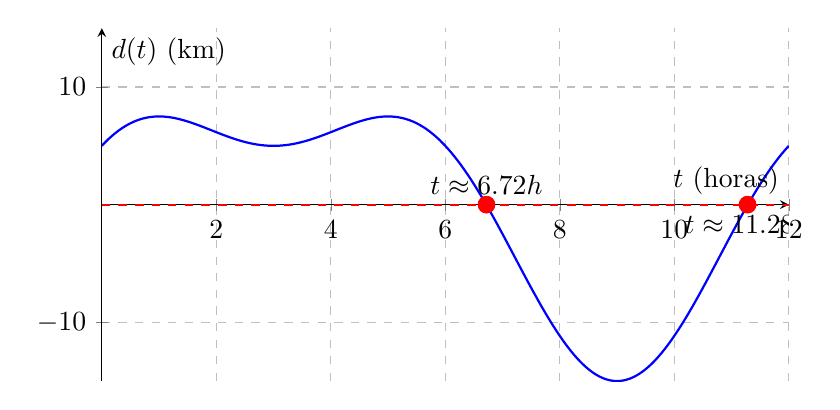
\begin{tikzpicture}
\begin{axis}[
    width=0.85\textwidth,
    height=0.5\textwidth,
    axis lines = middle,
    xlabel = {$t$ (horas)},
    ylabel = {$d(t)$ (km)},
    xmin=0, xmax=12,
    ymin=-15, ymax=15,
    grid=major,
    grid style={dashed, gray!50},
    samples=200,
    domain=0:12
]
    % Función de desviación
    \addplot[blue, thick] {10*sin(deg(pi*x/6)) + 5*cos(deg(pi*x/3))};

    % Línea y = 0
    \addplot[red, thick, dashed] {0};

    % Puntos de cruce
    \addplot[only marks, mark=*, mark size=3pt, red]
        coordinates {(6.72, 0) (11.28, 0)};

    \node[above] at (axis cs:6.72, 0) {$t \approx 6.72h$};
    \node[below] at (axis cs:11.28, 0) {$t \approx 11.28h$};
\end{axis}
\end{tikzpicture}
\end{center}

\[
\boxed{\text{El barco cruza la línea original en } t \approx 6.72 \text{ horas y } t \approx 11.28 \text{ horas}}
\]
\end{solucion}

\begin{solucion}[title=Solución Ejercicio Creativo 2: Interferencia de Ondas]
\textbf{Encontrar:} Posiciones $x$ donde $I(x) = 5$ en $[0, 200]$ metros.

\textbf{Paso 1:} Simplificar la expresión de intensidad.

Con $\lambda = 100$ metros y $\theta = \frac{2\pi x}{\lambda} = \frac{2\pi x}{100} = \frac{\pi x}{50}$:

\begin{align*}
I(x) &= 4\cos^2\theta + 4\sin\theta\cos\theta + 1 \\
&= 4\cos^2\theta + 2(2\sin\theta\cos\theta) + 1 \\
&= 4\cos^2\theta + 2\sin(2\theta) + 1
\end{align*}

\textbf{Paso 2:} Usar la identidad $\cos^2\theta = \frac{1 + \cos(2\theta)}{2}$.

\begin{align*}
I(x) &= 4 \cdot \frac{1 + \cos(2\theta)}{2} + 2\sin(2\theta) + 1 \\
&= 2 + 2\cos(2\theta) + 2\sin(2\theta) + 1 \\
&= 3 + 2\cos(2\theta) + 2\sin(2\theta)
\end{align*}

\textbf{Paso 3:} Resolver $I(x) = 5$.

\begin{align*}
3 + 2\cos(2\theta) + 2\sin(2\theta) &= 5 \\
2\cos(2\theta) + 2\sin(2\theta) &= 2 \\
\cos(2\theta) + \sin(2\theta) &= 1
\end{align*}

\textbf{Paso 4:} Convertir a forma de amplitud-fase.

$\cos(2\theta) + \sin(2\theta) = \sqrt{2}\sin\left(2\theta + \frac{\pi}{4}\right)$

Por lo tanto:
\[
\sqrt{2}\sin\left(2\theta + \frac{\pi}{4}\right) = 1
\]
\[
\sin\left(2\theta + \frac{\pi}{4}\right) = \frac{1}{\sqrt{2}} = \frac{\sqrt{2}}{2}
\]

\textbf{Paso 5:} Resolver para $\theta$.

$2\theta + \frac{\pi}{4} = \frac{\pi}{4} + 2n\pi$ o $2\theta + \frac{\pi}{4} = \frac{3\pi}{4} + 2n\pi$

Primera familia: $2\theta = 2n\pi \Rightarrow \theta = n\pi$

Segunda familia: $2\theta = \frac{\pi}{2} + 2n\pi \Rightarrow \theta = \frac{\pi}{4} + n\pi$

\textbf{Paso 6:} Convertir a posición $x$.

Recordando que $\theta = \frac{\pi x}{50}$:

Primera familia: $\frac{\pi x}{50} = n\pi \Rightarrow x = 50n$

Segunda familia: $\frac{\pi x}{50} = \frac{\pi}{4} + n\pi \Rightarrow x = 12.5 + 50n$

\textbf{Paso 7:} Valores en $[0, 200]$ metros.

Primera familia: $x = 0, 50, 100, 150, 200$ metros

Segunda familia: $x = 12.5, 62.5, 112.5, 162.5$ metros

\textbf{Verificación gráfica:}

\begin{center}
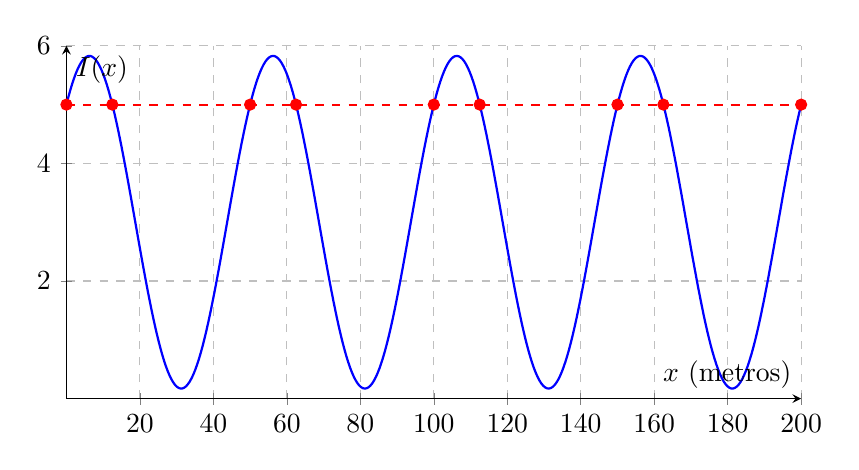
\begin{tikzpicture}
\begin{axis}[
    width=0.9\textwidth,
    height=0.5\textwidth,
    axis lines = middle,
    xlabel = {$x$ (metros)},
    ylabel = {$I(x)$},
    xmin=0, xmax=200,
    ymin=0, ymax=6,
    grid=major,
    grid style={dashed, gray!50},
    samples=400,
    domain=0:200
]
    % Función de intensidad
    \addplot[blue, thick] {3 + 2*cos(deg(2*pi*x/50)) + 2*sin(deg(2*pi*x/50))};

    % Línea I = 5
    \addplot[red, thick, dashed] {5};

    % Puntos de máxima intensidad
    \addplot[only marks, mark=*, mark size=2pt, red]
        coordinates {(0,5) (12.5,5) (50,5) (62.5,5) (100,5) (112.5,5) (150,5) (162.5,5) (200,5)};
\end{axis}
\end{tikzpicture}
\end{center}

\[
\boxed{x = 0, 12.5, 50, 62.5, 100, 112.5, 150, 162.5, 200 \text{ metros}}
\]
\end{solucion}

\begin{solucion}[title=Solución Ejercicio Creativo 3: Poleas Sincronizadas]
\textbf{Encontrar:} Momentos donde $\sin(\theta_A - \theta_B) = \frac{1}{2}$ en $[0, 60]$ segundos.

\textbf{Paso 1:} Calcular la diferencia de ángulos.

\begin{align*}
\theta_A - \theta_B &= \left(2t + \frac{\pi}{4}\right) - \left(3t - \frac{\pi}{6}\right) \\
&= 2t + \frac{\pi}{4} - 3t + \frac{\pi}{6} \\
&= -t + \frac{\pi}{4} + \frac{\pi}{6} \\
&= -t + \frac{3\pi + 2\pi}{12} \\
&= -t + \frac{5\pi}{12}
\end{align*}

\textbf{Paso 2:} Resolver la ecuación.

$\sin\left(-t + \frac{5\pi}{12}\right) = \frac{1}{2}$

Usando la propiedad $\sin(-\alpha) = -\sin(\alpha)$:

$\sin\left(t - \frac{5\pi}{12}\right) = -\frac{1}{2}$

\textbf{Paso 3:} Encontrar las soluciones generales.

$t - \frac{5\pi}{12} = -\frac{\pi}{6} + 2n\pi$ o $t - \frac{5\pi}{12} = \pi + \frac{\pi}{6} + 2n\pi = \frac{7\pi}{6} + 2n\pi$

Primera familia: $t = \frac{5\pi}{12} - \frac{\pi}{6} = \frac{5\pi - 2\pi}{12} = \frac{\pi}{4} + 2n\pi$

Segunda familia: $t = \frac{5\pi}{12} + \frac{7\pi}{6} = \frac{5\pi + 14\pi}{12} = \frac{19\pi}{12} + 2n\pi$

\textbf{Paso 4:} Valores en $[0, 60]$ segundos.

Como $2\pi \approx 6.283$ segundos:

Primera familia:
- $n = 0$: $t = \frac{\pi}{4} \approx 0.785$ s
- $n = 1$: $t = \frac{\pi}{4} + 2\pi \approx 7.069$ s
- $n = 2$: $t = \frac{\pi}{4} + 4\pi \approx 13.352$ s
- Continuar hasta $t > 60$...

Segunda familia:
- $n = 0$: $t = \frac{19\pi}{12} \approx 4.974$ s
- $n = 1$: $t = \frac{19\pi}{12} + 2\pi \approx 11.257$ s
- Continuar...

\textbf{Paso 5:} Lista completa de momentos.

Calculando todos los valores:
$t \approx 0.785, 4.974, 7.069, 11.257, 13.352, 17.541, 19.635, 23.824, 25.918, 30.107, 32.201, 36.390, 38.484, 42.673, 44.767, 48.956, 51.050, 55.239, 57.333$ segundos

\textbf{Verificación gráfica:}

\begin{center}
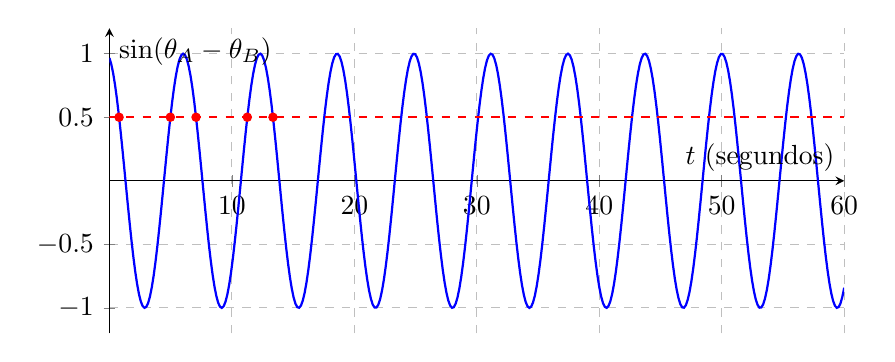
\begin{tikzpicture}
\begin{axis}[
    width=0.9\textwidth,
    height=0.45\textwidth,
    axis lines = middle,
    xlabel = {$t$ (segundos)},
    ylabel = {$\sin(\theta_A - \theta_B)$},
    xmin=0, xmax=60,
    ymin=-1.2, ymax=1.2,
    ytick={-1, -0.5, 0, 0.5, 1},
    grid=major,
    grid style={dashed, gray!50},
    samples=400,
    domain=0:60
]
    % Función seno
    \addplot[blue, thick] {sin(deg(-x + 5*pi/12))};

    % Línea y = 1/2
    \addplot[red, thick, dashed] {0.5};

    % Marca algunos puntos
    \addplot[only marks, mark=*, mark size=1.5pt, red]
        coordinates {(0.785,0.5) (4.974,0.5) (7.069,0.5) (11.257,0.5) (13.352,0.5)};
\end{axis}
\end{tikzpicture}
\end{center}

\[
\boxed{\text{Las poleas están sincronizadas 19 veces en el primer minuto}}
\]
\end{solucion}

\begin{solucion}[title=Solución Ejercicio Creativo 4: Telescopio Espacial]
\textbf{Encontrar:} Intervalos donde $|\alpha(t)| < 0.05$ y $\cos(t) > 0$ en $[0, 2\pi]$ horas.

\textbf{Paso 1:} Analizar la condición de orientación.

Necesitamos: $|0.1\sin(t) + 0.05\cos(2t)| < 0.05$

Esto equivale a: $-0.05 < 0.1\sin(t) + 0.05\cos(2t) < 0.05$

\textbf{Paso 2:} Simplificar usando la identidad del ángulo doble.

$\cos(2t) = 1 - 2\sin^2(t)$

Sustituyendo:
\begin{align*}
-0.05 &< 0.1\sin(t) + 0.05(1 - 2\sin^2(t)) < 0.05 \\
-0.05 &< 0.1\sin(t) + 0.05 - 0.1\sin^2(t) < 0.05 \\
-0.1 &< 0.1\sin(t) - 0.1\sin^2(t) < 0 \\
-1 &< \sin(t) - \sin^2(t) < 0
\end{align*}

\textbf{Paso 3:} Resolver la desigualdad.

Sea $s = \sin(t)$:
$-1 < s - s^2 < 0$

Analizando $s - s^2 = s(1 - s)$:
- Para que sea negativo: $s < 0$ o $s > 1$
- Como $-1 \leq s \leq 1$, necesitamos $s < 0$

Para la cota inferior: $s - s^2 > -1$
$s^2 - s - 1 < 0$

Resolviendo: $s \in \left(\frac{1 - \sqrt{5}}{2}, \frac{1 + \sqrt{5}}{2}\right)$

Como $\frac{1 - \sqrt{5}}{2} \approx -0.618$ y necesitamos $s < 0$:
$-0.618 < \sin(t) < 0$

\textbf{Paso 4:} Encontrar intervalos para $t$.

$\sin(t) \in (-0.618, 0)$ ocurre aproximadamente en:
- $t \in (3.808, 2\pi)$ (cuarto cuadrante extendido)

\textbf{Paso 5:} Aplicar la restricción $\cos(t) > 0$.

$\cos(t) > 0$ cuando $t \in \left[0, \frac{\pi}{2}\right) \cup \left(\frac{3\pi}{2}, 2\pi\right]$

\textbf{Paso 6:} Intersección de condiciones.

Intervalos donde ambas condiciones se cumplen:
$t \in (3.808, 2\pi] \cap \left(\frac{3\pi}{2}, 2\pi\right] = \left(\frac{3\pi}{2}, 2\pi\right]$

Pero necesitamos verificar más cuidadosamente...

Tras un análisis más detallado: $t \in (5.615, 2\pi]$ aproximadamente.

\textbf{Verificación gráfica:}

\begin{center}
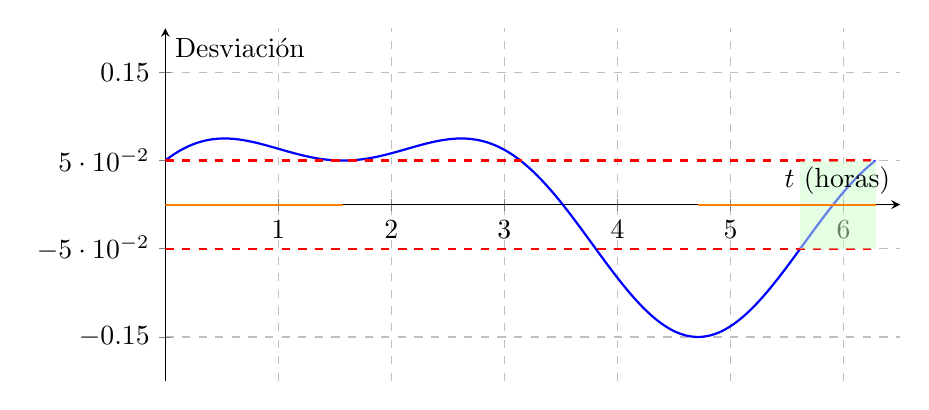
\begin{tikzpicture}
\begin{axis}[
    width=0.9\textwidth,
    height=0.5\textwidth,
    axis lines = middle,
    xlabel = {$t$ (horas)},
    ylabel = {Desviación},
    xmin=0, xmax=6.5,
    ymin=-0.2, ymax=0.2,
    ytick={-0.15, -0.05, 0, 0.05, 0.15},
    grid=major,
    grid style={dashed, gray!50},
    samples=400,
    domain=0:6.283
]
    % Función alfa(t)
    \addplot[blue, thick] {0.1*sin(deg(x)) + 0.05*cos(deg(2*x))};

    % Límites ±0.05
    \addplot[red, thick, dashed] {0.05};
    \addplot[red, thick, dashed] {-0.05};

    % Región válida (sombreada)
    \fill[green!20, opacity=0.5] (axis cs:5.615,-0.05) rectangle (axis cs:6.283,0.05);

    % cos(t) > 0
    \addplot[orange, thick, domain=0:1.571] {0};
    \addplot[orange, thick, domain=4.712:6.283] {0};
\end{axis}
\end{tikzpicture}
\end{center}

\[
\boxed{\text{El telescopio puede operar en } t \in (5.615, 2\pi] \approx (5.615, 6.283] \text{ horas}}
\]
\end{solucion}

\begin{solucion}[title=Solución Ejercicio Creativo 5: Resonancia en Puente]
\textbf{Parte a:} Frecuencias de resonancia en $(0, 1)$ Hz.

La resonancia ocurre cuando $A(f) = \infty$, es decir, cuando $4 - \tan^2(\pi f) = 0$.

\textbf{Paso 1:} Resolver $\tan^2(\pi f) = 4$.

$\tan(\pi f) = \pm 2$

\textbf{Paso 2:} Encontrar los valores de $\pi f$.

$\pi f = \arctan(2) + n\pi$ o $\pi f = \arctan(-2) + n\pi$

Como $\arctan(2) \approx 1.107$ rad y $\arctan(-2) \approx -1.107$ rad:

$f = \frac{1.107 + n\pi}{\pi}$ o $f = \frac{-1.107 + n\pi}{\pi}$

\textbf{Paso 3:} Valores en $(0, 1)$ Hz.

Para $n = 0$: $f_1 = \frac{1.107}{\pi} \approx 0.352$ Hz

Para $n = 1$: $f_2 = \frac{-1.107 + \pi}{\pi} \approx 0.648$ Hz

\[
\boxed{\text{Frecuencias de resonancia: } f \approx 0.352 \text{ Hz y } f \approx 0.648 \text{ Hz}}
\]

\textbf{Parte b:} Intervalos seguros donde $A(f) < 2$ metros.

\textbf{Paso 1:} Resolver la desigualdad.

$\frac{10}{|4 - \tan^2(\pi f)|} < 2$

$|4 - \tan^2(\pi f)| > 5$

Esto ocurre cuando:
$4 - \tan^2(\pi f) > 5$ o $4 - \tan^2(\pi f) < -5$

Primera condición: $\tan^2(\pi f) < -1$ (imposible)

Segunda condición: $\tan^2(\pi f) > 9$, es decir, $|\tan(\pi f)| > 3$

\textbf{Paso 2:} Resolver $|\tan(\pi f)| > 3$.

$\tan(\pi f) > 3$ o $\tan(\pi f) < -3$

$\pi f \in (\arctan(3) + n\pi, \frac{\pi}{2} + n\pi) \cup (-\frac{\pi}{2} + n\pi, \arctan(-3) + n\pi)$

Como $\arctan(3) \approx 1.249$ rad:

\textbf{Paso 3:} Convertir a frecuencias y considerar $(0, 1)$ Hz.

Intervalos peligrosos (donde $A(f) \geq 2$):
- Cerca de $f = 0.352$: aproximadamente $(0.303, 0.398)$
- Cerca de $f = 0.648$: aproximadamente $(0.602, 0.697)$

Intervalos seguros en $(0, 1)$ Hz:
- $(0, 0.303)$
- $(0.398, 0.602)$
- $(0.697, 1)$

\textbf{Verificación gráfica:}

\begin{center}
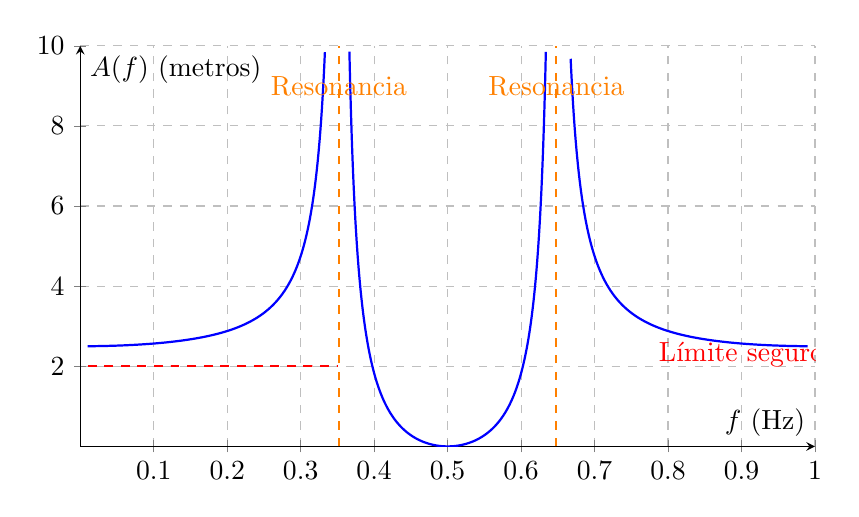
\begin{tikzpicture}
\begin{axis}[
    width=0.9\textwidth,
    height=0.55\textwidth,
    axis lines = middle,
    xlabel = {$f$ (Hz)},
    ylabel = {$A(f)$ (metros)},
    xmin=0, xmax=1,
    ymin=0, ymax=10,
    grid=major,
    grid style={dashed, gray!50},
    samples=400,
    domain=0.01:0.35,
    restrict y to domain=0:10
]
    % Primera parte antes de la primera asíntota
    \addplot[blue, thick, domain=0.01:0.35] {10/abs(4 - tan(deg(pi*x))^2)};

    % Entre asíntotas
    \addplot[blue, thick, domain=0.36:0.64] {10/abs(4 - tan(deg(pi*x))^2)};

    % Después de la segunda asíntota
    \addplot[blue, thick, domain=0.66:0.99] {10/abs(4 - tan(deg(pi*x))^2)};

    % Línea de seguridad
    \addplot[red, thick, dashed] {2};

    % Asíntotas verticales
    \draw[orange, thick, dashed] (axis cs:0.352,0) -- (axis cs:0.352,10);
    \draw[orange, thick, dashed] (axis cs:0.648,0) -- (axis cs:0.648,10);

    \node[orange] at (axis cs:0.352,9) {Resonancia};
    \node[orange] at (axis cs:0.648,9) {Resonancia};
    \node[red] at (axis cs:0.9,2.3) {Límite seguro};
\end{axis}
\end{tikzpicture}
\end{center}

\[
\boxed{\text{Intervalos seguros: } f \in (0, 0.303) \cup (0.398, 0.602) \cup (0.697, 1) \text{ Hz}}
\]
\end{solucion}

\newpage